\section{Sensor}
Sensoren der anvedes er en "Line Sensor Breakout - QRE1113" fra sparkfun.com. Det er en analog sensor som sidder på et breakout board i en spændingsdeling. Dette betyder at der blot skal aflæses spænding på en pin for at få en værdi der svarer til en lysstyrke fra sensoren.

\begin{figure}[h!]
  \centering
  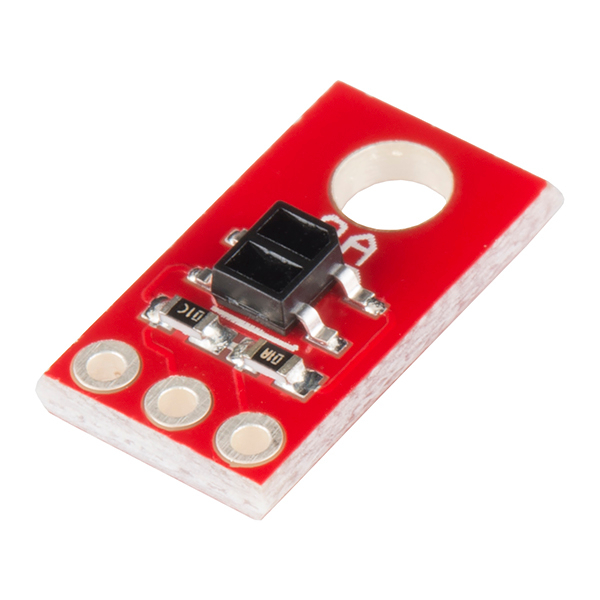
\includegraphics[width=0.3\textwidth]{figures/lyssensor.png}
\end{figure}

Specifikationerne gældende for sensoren: 
\begin{itemize}  
\item 5VDC operating voltage 
\item 25mA supply current
\item Optimal sensing distance: 0.125" (3mm) 
\item Dimension: 0.30 x 0.55 “ (7.62 x 13.97 mm)
\end{itemize}

Kilde (Sparkfun.com)
\newline
For at kunne anvende lyssensoren med en arduino skal noget software skrives. Sensoren sidder i en spændingsdeling og outputtet fra lyssensoren tilkobles en pin på arduinoen.
Herfra foretages en analog måling med ADC'en (analog til digital konverter) på arduinoen. Dette gøres ved at anvende analogRead() i softwaren.
\newline
I sensorens spændingsdeling sidder en transistor som generere høj frekvens støj. For at filtrere støjen væk anvendes et low-pass filter.
\newline
